%!TEX root = ../thesis.tex
%Adding the above line, with the name of your base .tex file (in this case "thesis.tex") will allow you to compile the whole thesis even when working inside one of the chapter tex files

\chapter{Appendix}

\label{app:1}

%If we assume the herringbones are due to the shock drift acceleration process then the velocity upon a reflection from the shock is
%\begin{equation}
%v_{r,||} = 2v_{shock}\mathrm{sec}\,\theta_{Bn} - v_{i,||}
%\end{equation}
%where $v_{r,||}$ is the reflected parallel velocity of the particle, $v_{i,||}$ is the incident parallel velocity of the paticle, $v_{shock}$ is the shock velocity, and $\theta$ is the angle between upstream $B-$field and shock normal $n$. Taking the shock speed to be the speed of the 150\,MHz radio source, $550\times10^3$\,m\,s$^{-1}$, and $v_{i,||}$ to be the thermal speed of an electron 
%\begin{equation} 
%v_{thermal} = \sqrt{ \frac{3k_bT}{m_e} }
%\end{equation}
%At $1\times10^{6}$\,K, $v_{thermal} = v_{i,||} = 6.7\times10^6$\,m\,s$^{-1}$. Now, the herringbone electron speed 0.15\,c, this is the reflected speed $v_{r,||}$ in equation A1. Rearranging A1 we get
%\begin{equation}
%\theta_{Bn} = \mathrm{sec}^{-1}\bigg( \frac{1}{2}\frac{v_{r,||} +  v_{i,||} }{v_{shock}}\bigg)
%\end{equation}
%Substituting the above values we get $\theta_{Bn}=88^{\circ}$. Independent verification of a quasi-perpendicular shock orientation!



\section{Radio Burst Emissivity}\label{app:emissivity}
The full equations for emissivity of EM waves from the stochastic growth theory are
\begin{equation}
j_M(r) \approx \frac{\Phi_M}{\Delta\Omega_M}\frac{n_b m_e v_b^3}{3l(r)}\frac{\Delta v_b}{v_b}
\label{eqn:plasma_emiss}
\end{equation}

\begin{equation}
\Phi_F \approx 72\sqrt{3}   \frac{\gamma_{L^{'}}}{\gamma_S}   \frac{v_e^3}{c^3}   \frac{v_b}{\Delta v_b}   \frac{e^{-u_c^2}}{u_c\sqrt{\pi}}  \zeta_F
\end{equation}
\begin{equation}
\Phi_H \approx \frac{18\sqrt{3}}{5\gamma_t}   \sqrt{\frac{m_i}{\gamma_t m_e}}  \frac{v_e^3 v_b^3}{c^5} \frac{v_b}{\Delta v_b}\zeta_H
\end{equation}
the expression involving $u_c$ represent an \textquoteleft escape factor' for the fundamental taking into account absorption and scattering of the radiation. $ \frac{\gamma_{L^{'}}}{\gamma_S} $ is the ratio of the damping rates of the product waves out of processes in equations~\ref{eqn:harm} and \ref{eqn:fund}. The $\zeta$ terms are the fractions of Langmuir waves that are kinematically able to contribute to the fundamental or harmonic emission, given by

\begin{equation}
\zeta_F  \approx \mathrm{exp} \bigg[  -\frac{4\gamma_t m_e}{45 m_i}    \bigg(\frac{v_b}{\Delta v_b}\bigg)^2   \bigg(  \frac{3}{2}  \sqrt{\frac{m_i}{\gamma_t m_e}} - \frac{v_b}{v_e}  \bigg)^2    \bigg]
\end{equation}

\begin{equation}
\zeta_H \approx \frac{c}{2v_b} \sqrt{\frac{\pi}{6}} \frac{\beta \Delta v_b}{v_b}
\Bigg[  \mathrm{erf}\Bigg(     \frac{ \frac{v_e\sqrt{3}}{c}  + \frac{2}{3} \sqrt{\frac{\gamma_t m_e}{m_i}}  }  {\frac{v_e}{v_b} \frac{\beta \Delta v_b}{v_b} \sqrt{2} }   \Bigg)     +   \mathrm{erf}\Bigg(     \frac{ \frac{v_e\sqrt{3}}{c}  - \frac{2}{3} \sqrt{\frac{\gamma_t m_e}{m_i}}  }  {\frac{v_e}{v_b} \frac{\beta \Delta v_b}{v_b} \sqrt{2} }   \Bigg)   \Bigg]
\end{equation}
where erf is the error function \citep{robinson1993a, robinson1998}. 

\section{EUV and pB Density Measurements}\label{app:densities}

Electron densities were calculated from emission measure maps derived using the SDO/AIA�s six coronal filters and the method of \citep{asch2013}. The method starts by reconstructing the differential emission measure $dEM/dT (DEM)$, using the intensity of the six SDO/AIA filters for each pixel. The DEM is a measure of the amount of plasma along the line-of-sight (LOS) that contributes to the emitted radiation in the temperature range $T$ to $T +dT$ \citep{craig1976}. Once the EM was obtained, the plasma electron density can be calculated estimating an effective length of the LOS of the emitting plasma. The 2D $EM(r, \phi)$ map, which is a function of heliocentric distance $r$ and latitude, can then be written as
\begin{eqnarray}
EM(r, \phi) &=& \int \bigg( \frac{dEM(r,\phi)}{dT} \bigg) dT \\
			  &=& \int <N_e^2> ds
\end{eqnarray}

Knowing the line-of-sight length, $s$, the density of the emitting plasma can be obtained from the EM,
\begin{equation}
N_e(r, \phi) =\sqrt{  \frac{EM(r, \phi)}{s(r)}  }
\end{equation}
The LOS length was calculated using a geometrical method used widely in stellar atmospheres \citep{menzel1936}. The LOS length s changes at different distance $r$ and contributes to the intensity of the emitting plasma measured by the observer. This gives the LOS using an asymptotic series expansion in the form
\begin{equation}
S\approx \sqrt{H\pi r}
\end{equation}
where $H$ is the scale height. Using a typical coronal temperature of 2\,MK the scale height $H$ is of the order of $9\times10^9$\,cm and the LOS is in the order of $4\times10^{10}$\,cm. The LOS length does not change significantly in the 1--1.3\,$R_{\odot}$ range. 

As for the polarized brightness measurements, the density diagnostic is through the use of coronagraph images and the Thomson scattering theory outlines in Chaoter. The method involves using the coronagraph data to extract polarized brightness measurements as a function of height i.e., along a radial trace in the coronagraph images. A polynomial is then fit to this data
\begin{equation}
I_t - I_r =\sum_s k_s x^{-s}
\end{equation} 
where $I_t - I_r$ is the polarized brightness, and $x$ is the radial position in the corona, $r$, projected onto the plane of sky. \citet{vdeh50} showed that by use of the van de Hulst coefficients the electron density along the same radial trace can be expressed as 
\begin{equation}
N(r) = \frac{1}{C\{A(r) - B(r)\}}\sum_s \frac{k_s}{a_{s+1}} r^{-s} \, \,\,\,\,\, \textrm{where} \,\,\,\,\, a_n=\frac{\pi}{2^{n+1}}\frac{n!}{(1/2n!)^2}
\end{equation}
here $C$ is constant equal to $\frac{3}{4}\times1R_{\odot}\times \sigma_T$; $\sigma_T$ is the Thomson scattering cross section and $A(r)$ and $B(r)$ are the van de Hulst coefficients (see Chapter 4). Here, the same $k_s$ produced from the polarized brightness fit are used to calculate $N(r)$. 
\vspace{5cm}
\section{June 7th 2011 Radio Burst from RSTO}\label{app:rsto_busrts}

The event of 7 June 2011 was an extremely complex eruption with a variety of associated radio activity (Figure~\ref{fig:june7}). The Callisto receivers at RSTO observed type II, type III, herringbones, and type IV. Also accompanying this activity was interplanetary type III bursts observed by STEREO WAVES in both Ahead and Behind spacecraft.
\begin{sidewaysfigure}[t!]
\centering
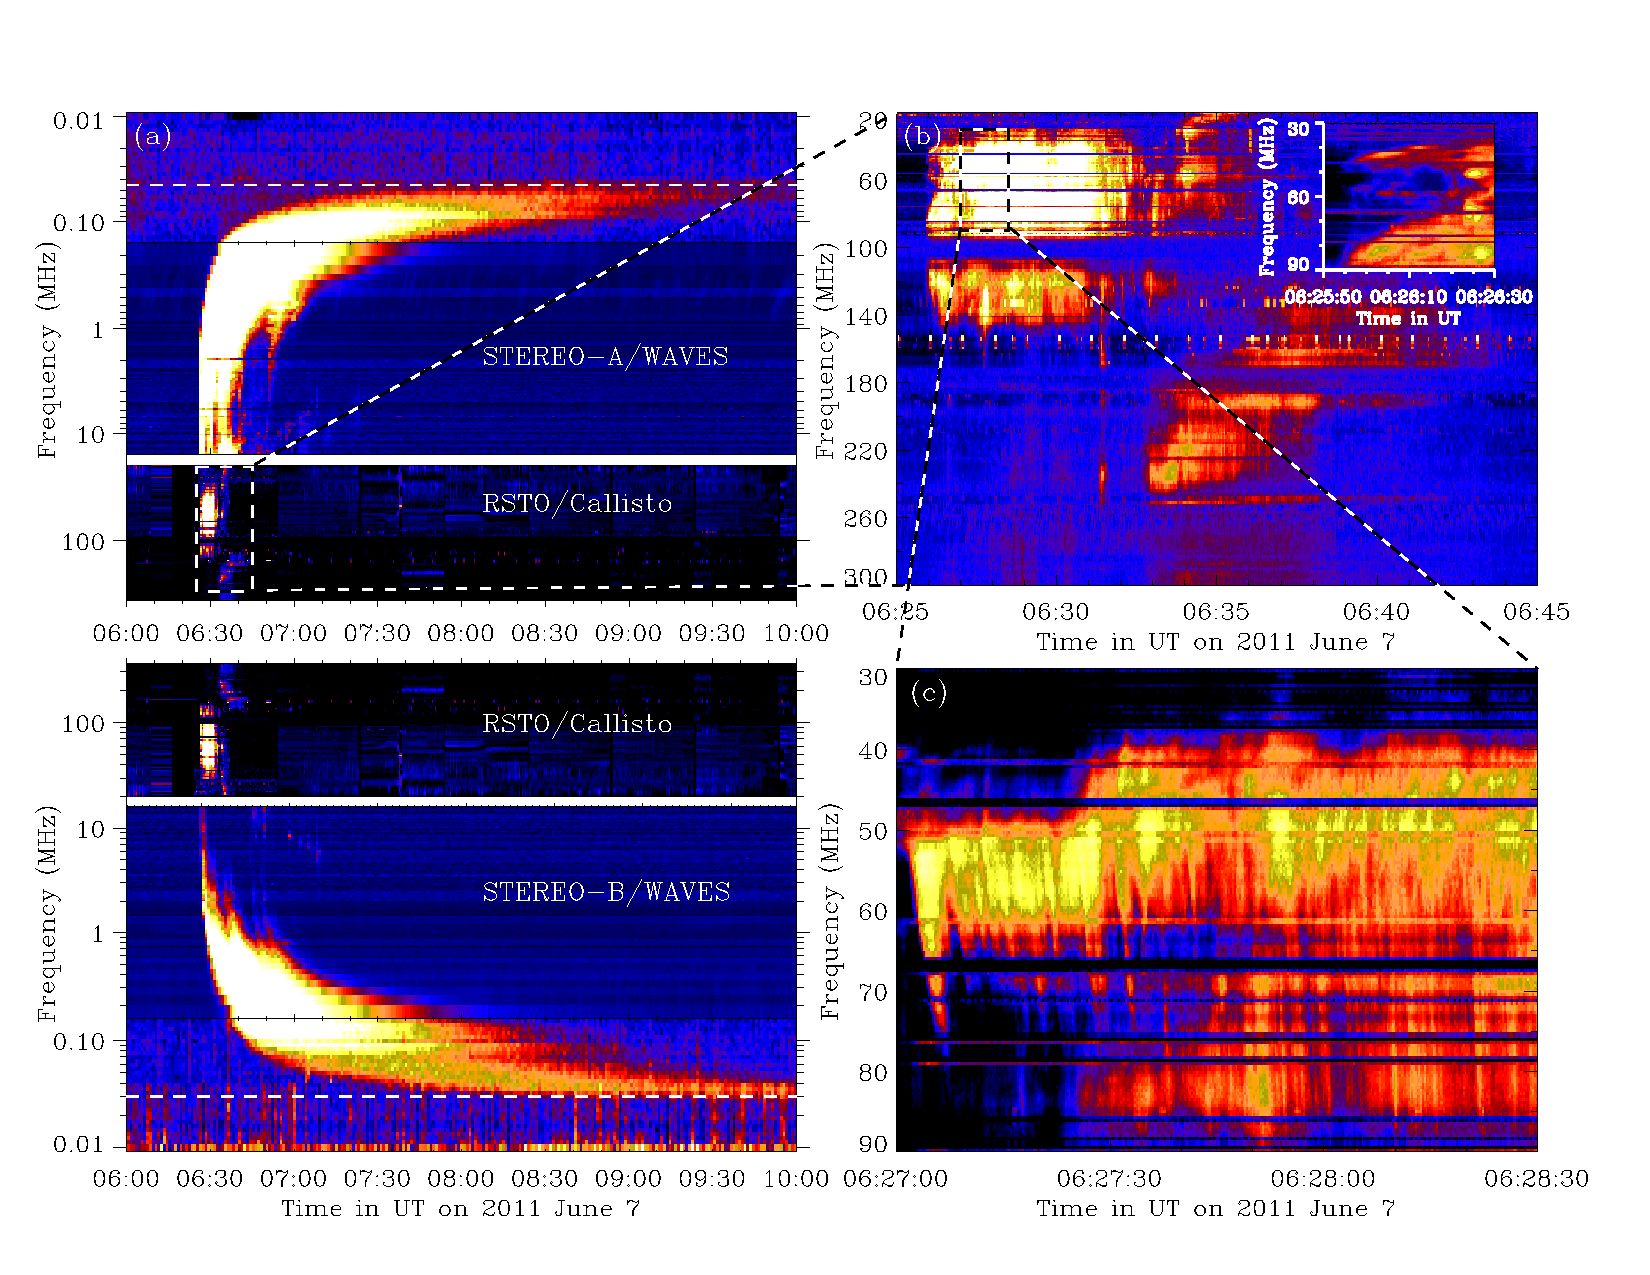
\includegraphics[scale=0.7, trim=0cm 1cm 0cm 1cm]{june7th_radio.pdf}
\caption{Radio activity detected by STEREO WAVES A and B and RSTO callisto spectrometers, observed on 7 June 2011. The radio activity was complex, with interplanetary type IIIs (a), a possible type II (inset of b), herringbones (c), and type IV (b).}
\label{fig:june7}
\end{sidewaysfigure}


